\documentclass[lettersize,journal]{IEEEtran} %这一行的作用是设置论文的格式,letterpaper表示纸张大小为美国信纸,journal表示论文类型为期刊论文,IEEEtran表示论文的格式为IEEEtran
\usepackage{amsmath,amsfonts} %这两个包分别是数学公式和数学字体的宏包
\usepackage{algorithm}
\usepackage{algpseudocode}
% \usepackage{algorithmic} %这个包是算法的宏包
\usepackage{array} %这个包是表格和数组的宏包
% \usepackage[caption=false,font=normalsize,labelfont=sf,textfont=sf]{subfig} %这个包是子图的宏包,它可以让你在一个图形环境中放置多个图形,可以对子图进行编号,可以对子图进行交叉引用,可以对子图进行标题设置
\usepackage{textcomp} %这个包是对文本模式下的符号进行扩展的宏包
\usepackage{stfloats} %这个包是控制双栏浮动图形和表格的宏包
\usepackage{url} %这个包是对网址进行扩展的宏包
\usepackage{verbatim} %这个包是对抄录环境进行扩展的宏包
\usepackage{graphicx} %这个包是对图形进行扩展的宏包
\usepackage{subcaption}
\usepackage{multirow}
\hyphenation{op-tical net-works semi-conduc-tor IEEE-Xplore} %这一行的作用是设置英文连字符,可以防止英文单词在换行时过长
\def\BibTeX{{\rm B\kern-.05em{\sc i\kern-.025em b}\kern-.08em
    T\kern-.1667em\lower.7ex\hbox{E}\kern-.125emX}} %这一行的作用是定义BibTeX的标志,这个标志在参考文献中会用到
\usepackage{balance} %这个包是平衡双栏文档最后一页的双栏高度的宏包



\begin{document} %这一行的作用是开始论文的正文部分
\title{GraphCPP: A Data-Driven System for Concurrent Point-to-Point Queries in Dynamic Graphs} %这一行的作用是设置论文的标题
\author{IEEE Publication Technology Department %这一行的作用是设置论文的作者
\thanks{Manuscript created October, 2020; This work was developed by the IEEE Publication Technology Department. This work is distributed under the \LaTeX \ Project Public License (LPPL) ( http://www.latex-project.org/ ) version 1.3. A copy of the LPPL, version 1.3, is included in the base \LaTeX \ documentation of all distributions of \LaTeX \ released 2003/12/01 or later. The opinions expressed here are entirely that of the author. No warranty is expressed or implied. User assumes all risk.}} %这一行的作用是设置论文的作者的单位和邮箱,这里的\thanks是设置脚注的命令

\markboth{Journal of \LaTeX\ Class Files,~Vol.~18, No.~9, September~2023}%这一行的作用是设置论文的页眉
{How to Use the IEEEtran \LaTeX \ Templates} 

\maketitle %它和title的区别是,title只是设置论文的标题,而maketitle是使论文的标题和作者的信息生效

\graphicspath{{E:/华科实验室论文/MyDocument/并发点对点查询/论文草稿/picture/}}


\begin{abstract} %这一行的作用是设置论文的摘要
With the widespread application of graph processing technology in fields such as map navigation and network analysis, there is a significant demand for high throughput in concurrent point-to-point query tasks on the same underlying graph. However, existing graph query systems have primarily focused on optimizing the speed of individual point-to-point queries. When dealing with concurrent query tasks, the overall throughput is compromised due to redundant data access overhead and computation expenses.

This paper introduces GraphCPP, the first graph traversal system designed for concurrent execution of point-to-point query tasks. It enhances the throughput of concurrent query tasks through data access sharing and hot path computation sharing. GraphCPP is novel in two ways. Firstly, based on the observation that traversal paths for different query tasks overlap significantly, GraphCPP proposes a data-driven caching execution mechanism.  Through fine-grained graph chunk scheduling, this mechanism enables data sharing among concurrent tasks, thereby enhancing data access efficiency. Secondly, recognizing the frequent computation of the same hot vertices and paths by distinct tasks, GraphCPP proposes a dual-level computation sharing mechanism. This mechanism accelerates the convergence of unknown queries by sharing computed values of hot vertices and paths. To demonstrate the efficiency of GraphCPP, we compare it with state-of-the-art point-to-point query systems such as SGraph, Tripoline, and Pnp on datasets like xx. The results indicate that GraphCPP incurs only xx preprocessing overhead and xx storage overhead, achieving a throughput improvement of xx-xx times.
  
\end{abstract}



\begin{IEEEkeywords}
graph process, point-to-point queries, concurrent jobs, data access similarity, computational similarity.
\end{IEEEkeywords}


\section{Introduction}
\IEEEPARstart{A} significant number of concurrent point-to-point query tasks are commonly executed on the same underlying graph. For instance, in logistics and transportation, Google Maps [xx] identifies the optimal route between two locations. In social network analysis, Facebook [x] recommends potential friends to users by exploring the relationship chain between two users. In financial risk analysis, Alipay [x] analyzes how risk spreads from one entity to another. These popular applications highlight the demand for executing large-scale concurrent point-to-point queries on the same underlying graph. However, existing solutions for point-to-point queries [xxxx] primarily focus on accelerating the efficiency of individual queries while neglecting optimization for concurrent queries. To achieve the efficient execution of concurrent point-to-point query tasks, two key challenges need to be addressed.


However, executing concurrent point-to-point query tasks on the same underlying graph without considering data access similarity leads to redundant access to overlapping data. Specifically, different query tasks start from distinct origins and eventually reach their respective destinations. There is a significant overlap in their traversal paths. However, as the overlapping portions of data accessed by different query tasks vary, and they traverse overlapping graph data along different paths. Therefore, existing query systems adopt a conservative strategy, assigning each task to access the data it requires independently. This means that the data access for each task is entirely isolated, even if their traversal paths highly overlap. For example, if the path of one query is a subset of the path of another query, the overlapping data needs to be loaded redundantly, preventing the benefits of reusing data in the cache.

Furthermore, in addition to redundant access, different query tasks also face the challenge of recalculating distance values for popular paths. As graph data often exhibits a power-law distribution, a small number of popular vertices frequently appear in the optimal paths of different queries. Due to the lack of computation sharing among different query tasks, they redundantly compute the hot paths connecting popular vertices. Moreover, popular vertices often correspond to high-degree vertices with numerous neighboring vertices, and the repetitive traversal of these vertices results in an explosive growth in computation costs. Some existing systems have attempted to implement computation sharing through global indexing [xxxx], but the efficiency and accuracy of computation sharing are limited by the expensive computational, storage, and update costs.

To address the challenges mentioned above, this paper proposes a data-driven concurrent point-to-point query system called GraphCPP. It enhances the throughput of concurrent point-to-point query systems through data sharing and computation sharing mechanisms.

In GraphCPP, we firstly introduce a data-driven caching execution mechanism that transforms the traditional $task→data$ scheduling approach into a $data→task$ scheduling approach, thereby enabling the sharing of overlapping graph structure data among multiple tasks. Under this execution mechanism, GraphCPP first determines the scheduling order of data: it logically partitions graph structure data into fine-grained chunks at the LLC level. Subsequently, it associates query tasks with the relevant graph chunks based on the graph block where the active vertices of the query tasks reside. The higher the number of associated tasks, the higher the priority for scheduling that chunk. As the set of active vertices changes in each round, and the number of associated tasks for shared chunks needs updating in each round, GraphCPP adopts an associated task-triggering mechanism to achieve $data→task$ scheduling. After loading the graph chunks into the LLC in priority order, the system utilizes the associated information obtained in each round to trigger the batch execution of associated tasks for the current chunk, efficiently accessing shared data.

Secondly, GraphCPP proposes a dual-level computation sharing mechanism comprising global indexing and core subgraph indexing. It designates vertices with a substantial number of connecting edges in the graph as hot vertices and the paths between hot vertices as hot paths. While the quantities of hot vertices and hot paths are limited, they frequently appear in traversal paths reached by different query tasks. The dual-level computation sharing mechanism achieves the first level of computation sharing through global indexing. The global index maintains a small set of hot vertices and their index information to other vertices. These hot vertices act as intermediary nodes for different query paths, providing prunable path values for the majority of queries. Through the core subgraph mechanism, the second level of computation sharing is realized. The core subgraph primarily maintains hot paths connecting hot vertices in the graph. It is essential to note that the number of hot vertices in the core subgraph is an order of magnitude larger than that in the global index. Specifically, it first filters hot vertices with high degrees from the original graph data. Subsequently, it traverses hot paths between these vertices, assigning the path values as weights to the edges between pairs of hot vertices. During the query process, the core subgraph functions like a high-speed highway network. The query task starts at a hot vertex (analogous to entering a highway at an entrance), proceeds to another hot vertex (similar to reaching an exit via the highway), and ultimately arrives at the destination vertex (analogous to reaching the destination from a highway exit). The dual-level computation sharing mechanism in GraphCPP reduces redundant computations.

Lastly, GraphCPP further enhances the performance of concurrent queries by predicting the traversal paths of different query tasks and driving the batch execution of highly overlapping similar query tasks.

This paper makes the following contributions:
\begin{enumerate}
  \item{We analyze the performance bottlenecks of existing point-to-point query systems when handling concurrent tasks and propose leveraging the similarities in data access and computation among concurrent tasks to enhance throughput.}
  \item{We develop GraphCPP, a dynamic graph-driven concurrent processing system for point-to-point queries. It achieves data sharing and computation sharing among concurrent tasks and introduces a strategy for batch execution of similar tasks.}
  \item{We compare GraphCPP with three state-of-the-art point-to-point query systems, namely XXXXXX, using a workload that includes x real-world graphs and x applications. Our experiments demonstrate that, on average, GraphCPP outperforms others, achieving xx times, xxx times, and xxx times improvement compared to XXX, XXX, and XXX, respectively.}
\end{enumerate}

\section{BACKGROUND AND MOTIVATION}
Most existing solutions [xxx] are primarily focused on accelerating the speed of individual queries. However, in practical scenarios, there is a significant number of graph query tasks concurrently running on the same underlying graph. For instance, statistics from CAGIS[xx] indicate that location service open platforms constructed by companies such as Baidu Maps[xx], Gaode Maps[xx], Tencent Maps[xx], and Huawei Maps[xx] receive a daily average of up to 160 billion location service requests. The substantial demand for concurrent point-to-point queries poses a high requirement for the throughput of graph traversal systems. Yet, as illustrated in table 1 (showing the parallel query execution time for different systems, highlighting poor parallel execution efficiency), we demonstrate that existing systems exhibit low throughput when handling large-scale concurrent queries. The root cause of this undesirable outcome is the significant redundancy in data access and computation among concurrent tasks. To qualitatively analyze the aforementioned issues, we conducted performance evaluations on parallel point-to-point queries using XXXXX (machine configuration), selecting XXXXX (the current best solution) on XXXXX (graph dataset).

\begin{figure}[!t]
    \centering
    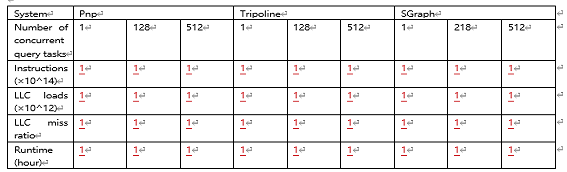
\includegraphics[width=\columnwidth]{system_compare.png}
    \caption{Your caption here}
    \label{fig:system_compare}
  \end{figure}


\subsection{Preliminaries}
Definition 1: ($Graph$) We use $G=(V,E)$ to denote a directed graph, where $V$ is the set of vertices, and $E$ is the set of directed edges formed by vertices in $V$ (for undirected graphs, edges can be split into two directed edges with different directions). We use $|V|$ and $|E|$ to represent the number of vertices and edges, respectively.

Definition 2: ($Graph~Partition$) We use $P_i=(V_{P_i},E_{P_i})$ to denote the $i_{th}  $ graph partition of a directed graph, where $V_{P_i}$ represents the set of vertices in the graph partition, and $E_{P_i}$ is the set of directed edges composed of vertices in $V_{P_i}$. In a distributed system, different machine-specific graph partitions $P_i$ are distinct. We partition the graph using edge cuts, where the same vertex may appear on different computing nodes, but there is only one primary vertex, while the others are mirror vertices.

Definition 3: ($Point \text{-} to \text{-} Point~Quer$y) We use $q_i=(s_i,d_i)$ to denote the query corresponding to task $i$, where $s_i$ and $d_i$ represent the source and destination vertices of query $q_i$, respectively. The result value $R_{s,d}$ obtained by query $q_i$ has different meanings for different algorithms; For example, in the case of the Shortest Optimal Path query, $R_{ib}$ represents the shortest optimal path between $s_i$ and $d_i$. We use $Q={q_1,q_2,\ldots,q_{|Q|}}$ to represent the set of concurrent point-to-point queries, where $|Q|$ indicates the total number of queries.

Definition 4: ($Bounds$) In mainstream point-to-point query systems, a pruning-based query strategy is widely adopted, where $bounds$ provide conservative pruning values. Specifically, $bounds$ can be further categorized into $upper~bounds$ ($UB$) and $lower~bounds$ ($LB$). $UB$ represents the current known optimal path value from the source to the destination vertex, while $LB$ signifies a conservative predicted distance value from the current vertex $v$ to the destination vertex, with the predicted $LB$ being less than or equal to the actual optimal distance from vertex $v$ to the destination vertex. Following the triangle inequality on the graph, if the distance of a path is greater than $UB$ or exceeds $UB$ when adding the value of $LB$, the path is definitely worse than existing paths and needs to be pruned. The values of upper and lower $bounds$ need indexing to be derived, essentially constituting a form of computation sharing.

Definition 5: ($Core~Subgraph$) We use $G_{core}=(V_{hot},E_{hot},Index_{hot})$ to represent the $core~subgraph$, where $V_{hot}$ is the set of $hot~vertices$ , $E_{hot}$ abstracts the $hot~paths$ between vertices in $V_{hot}$ as edges, and $Index_{hot}$ represents the path values corresponding to $E_{hot}$. A $hot vertex$ refers to a vertex in a graph with a significant number of edges. A $hot~path$ is defined as the optimal path between two $hot~vertices$. A $hot~index$ denotes the path value of a $hot~path$.

Definition 6: ($Index$) The $index$ records the optimal query path values between vertex pairs. GraphCPP sorts vertices by degree, selecting $k+m$ vertices with the highest degrees (values for $k$ and $m$ are generally user-determined, with $k$ usually set to 16, and $m$ typically one order of magnitude larger than $k$). The first $k$ vertices serve as $global~index$ vertices, while the remaining vertices function as $core~subgraph~ndex$ vertices. The $global~index$ records optimal query path values to all vertices in the graph. The $core~subgraph$ index only records query path values between hot vertices in the subgraph.

\begin{figure}[!t]
    \centering
  
    \begin{subfigure}{0.3\columnwidth}
      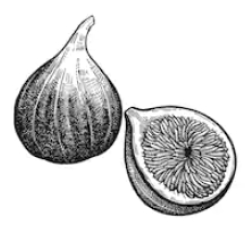
\includegraphics[width=\linewidth]{fig1.png}
      \caption{Caption for Subfigure 1}
      \label{fig:subfig1}
    \end{subfigure}
    \hfill
    \begin{subfigure}{0.3\columnwidth}
      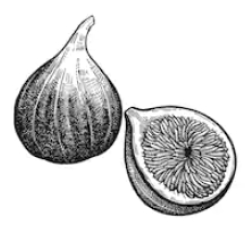
\includegraphics[width=\linewidth]{fig1.png}
      \caption{Caption for Subfigure 2}
      \label{fig:subfig2}
    \end{subfigure}
    \hfill
    \begin{subfigure}{0.3\columnwidth}
      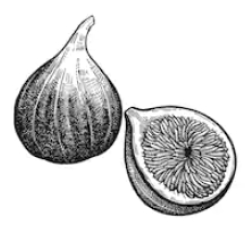
\includegraphics[width=\linewidth]{fig1.png}
      \caption{Caption for Subfigure 3}
      \label{fig:subfig3}
    \end{subfigure}
  
    \medskip
  
    \begin{subfigure}{0.3\columnwidth}
      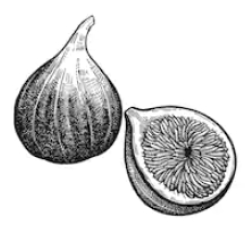
\includegraphics[width=\linewidth]{fig1.png}
      \caption{Caption for Subfigure 4}
      \label{fig:subfig4}
    \end{subfigure}
    \hfill
    \begin{subfigure}{0.3\columnwidth}
      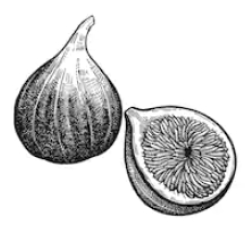
\includegraphics[width=\linewidth]{fig1.png}
      \caption{Caption for Subfigure 5}
      \label{fig:subfig5}
    \end{subfigure}
    \hfill
    \begin{subfigure}{0.3\columnwidth}
      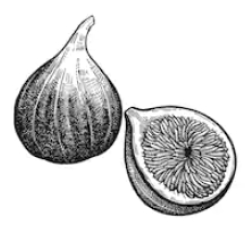
\includegraphics[width=\linewidth]{fig1.png}
      \caption{Caption for Subfigure 6}
      \label{fig:subfig6}
    \end{subfigure}
  
    \caption{Overall caption for the figure}
    \label{fig:overall}
  \end{figure}
  
  

\subsection{Performance Bottlenecks in Concurrent Point-to-Point Query Tasks}
In this section, we have developed the concurrent version SGraph-C based on the Gemini system, which is currently at the forefront of pairwise query systems. We evaluated the performance of SGraph-C in executing concurrent pairwise queries through Twitter, aiming to quantitatively illustrate the performance bottlenecks of existing concurrent pairwise query solutions.

{\bf{The redundant data access overhead of concurrent tasks is evident.}} We observe that when concurrent pairwise query tasks execute graph traversal on the same underlying graph, a significant portion of their traversal paths exhibits clear data access similarities. As shown in Figure 3x, our data indicates that there is a substantial overlap in data access among concurrent tasks, with a higher overlap ratio for similar tasks (more details are provided in Section xx). However, in the traditional "task->data" scheduling mode, different tasks independently execute queries, leading to competition for limited cache space to store their respective graph data chunks, even when these data chunks overlap. This results in severe cache thrashing and a reduction in the performance of processing concurrent pairwise queries. Table 1 illustrates that, with an increase in the number of concurrent tasks, the cache miss rate for query tasks sharply rises. Although the overall performance of concurrent execution surpasses linear execution, the average query time per task significantly increases with the growing number of query tasks due to the mentioned redundant data access overhead. It is essential to note that the total execution time in the concurrent mode is the maximum among the execution times of these tasks, while in the sequential mode, it is the sum of all task execution times.


{\bf{Redundant Computational Overhead of Concurrent Tasks.}}Due to the power-law distribution characteristics of graph data, a small number of hot vertices are connected to the majority of edges. Therefore, as shown in Figure 2, although hot vertices constitute only a small portion of the total vertices (XX\%), they appear in many paths (XX\%). The proportion of hot vertices in graph partitions with higher sharing levels is even higher. This implies that different query tasks will redundantly calculate hot paths between hot vertices, demonstrating computational similarity among concurrent tasks. Within a graph snapshot period, the results of path calculations for the same vertex pairs are identical, indicating that a significant amount of computation in concurrent tasks is redundant. Additionally, as illustrated in Figures 3 and 4, due to the fact that hot vertices often have a large number of outgoing and incoming edges, the computational cost they bring is much greater than that of ordinary vertices.

Some existing solutions attempt to establish a global indexing mechanism [x] to leverage computational similarity. However, the global indexing mechanism has inherent flaws. Flaw 1: Global indexing requires recording the path values between high-degree vertices and all other vertices. When the graph scale is extremely large, the computational and storage costs of building the index can be substantial, as shown in Figures 3 and 4, where the computational and storage costs of global indexing increase proportionally with the number of global index vertices. Flaw 2: In point-to-point queries on streaming graphs, each round of graph updates introduces new edges and edge deletions. The global index needs to dynamically update the index relationships between high-degree vertices and every vertex based on the latest graph snapshot. This implies that any update to the streaming graph will impact all vertex indices, as illustrated in Figure 5, where a small number of graph updates lead to extensive updates in the global index. Flaw 3: Different datasets have different data distribution patterns, making it challenging to choose an appropriate number of index vertices to balance the efficiency of computational sharing and the overhead of the index itself. As shown in Figure 6, selecting the same number of index vertices on different datasets results in significant variations in inherent costs and the effectiveness of computational sharing. In summary, the global indexing mechanism itself incurs expensive costs, and the fluctuation in required costs for different datasets is considerable. Therefore, existing systems often conservatively choose the number of global indices (e.g., 16 vertices in Tripoline and SGraph) to avoid incurring excessive costs. However, this also limits the coverage range of global indices, preventing efficient computational sharing. 



\subsection{Our Motivation}
Inspired by the observations mentioned above, we derive the following insights:

{\bf{Observation 1}}: There exists spatial similarity in data access among different query tasks. A significant portion of their traversal paths overlaps, but due to the asynchronous nature of accessing overlapping data by distinct tasks and the lack of support for data sharing between tasks in existing point-to-point query systems, redundant overhead is incurred in accessing overlapping data. This insight motivates the development of an efficient fine-grained data-sharing mechanism. By enabling different tasks to share access to the same data at different times, we aim to reduce data access overhead and enhance the throughput of concurrent queries.

{\bf{Observation 2}}: Computational similarity exists among different query tasks. The core subgraph composed of hot high-degree vertices and hot paths is akin to a highway network in road traffic systems, likely to be repeatedly traversed by various tasks. However, existing graph traversal systems either do not exploit computational similarity [xx pnp] or employ costly global indexing mechanisms [xx Tripoline], limiting the effectiveness of computational sharing. This observation inspires the establishment of a lightweight core subgraph mechanism to share hot path computation results across different query tasks. Different query paths can be seen as distinct lines, and high-degree vertices are the intersections of these lines, frequently appearing in various tasks. Existing global indexing methods are often expensive and tend to impose limits on the number of index vertices, resulting in a low proportion of shareable paths. This insight encourages the adoption of a lightweight indexing approach to achieve better computational sharing.

\section{GraphCPP Overview}

\subsection{System Architecture}
In order to enhance the execution efficiency of concurrent point-to-point queries, we propose a data-driven and efficient concurrent point-to-point query system, GraphCPP, after a meticulous examination of the computational intricacies of concurrent point-to-point queries. The fundamental concept of our system is to achieve data and computation sharing among concurrent point-to-point query tasks. As depicted in the figure below, GraphCPP incorporates an efficient data-driven caching execution mechanism. It exploits data similarity among concurrent tasks to facilitate shared access to overlapping data. Additionally, it introduces a dual-level computation sharing mechanism based on the core subgraph, enabling the sharing of computations for the same hot paths across different query tasks. Moreover, it employs path prediction for different queries, driving the bulk execution of similar queries with overlapping paths and further leveraging data similarity.

\begin{figure}[!t]
    \centering
    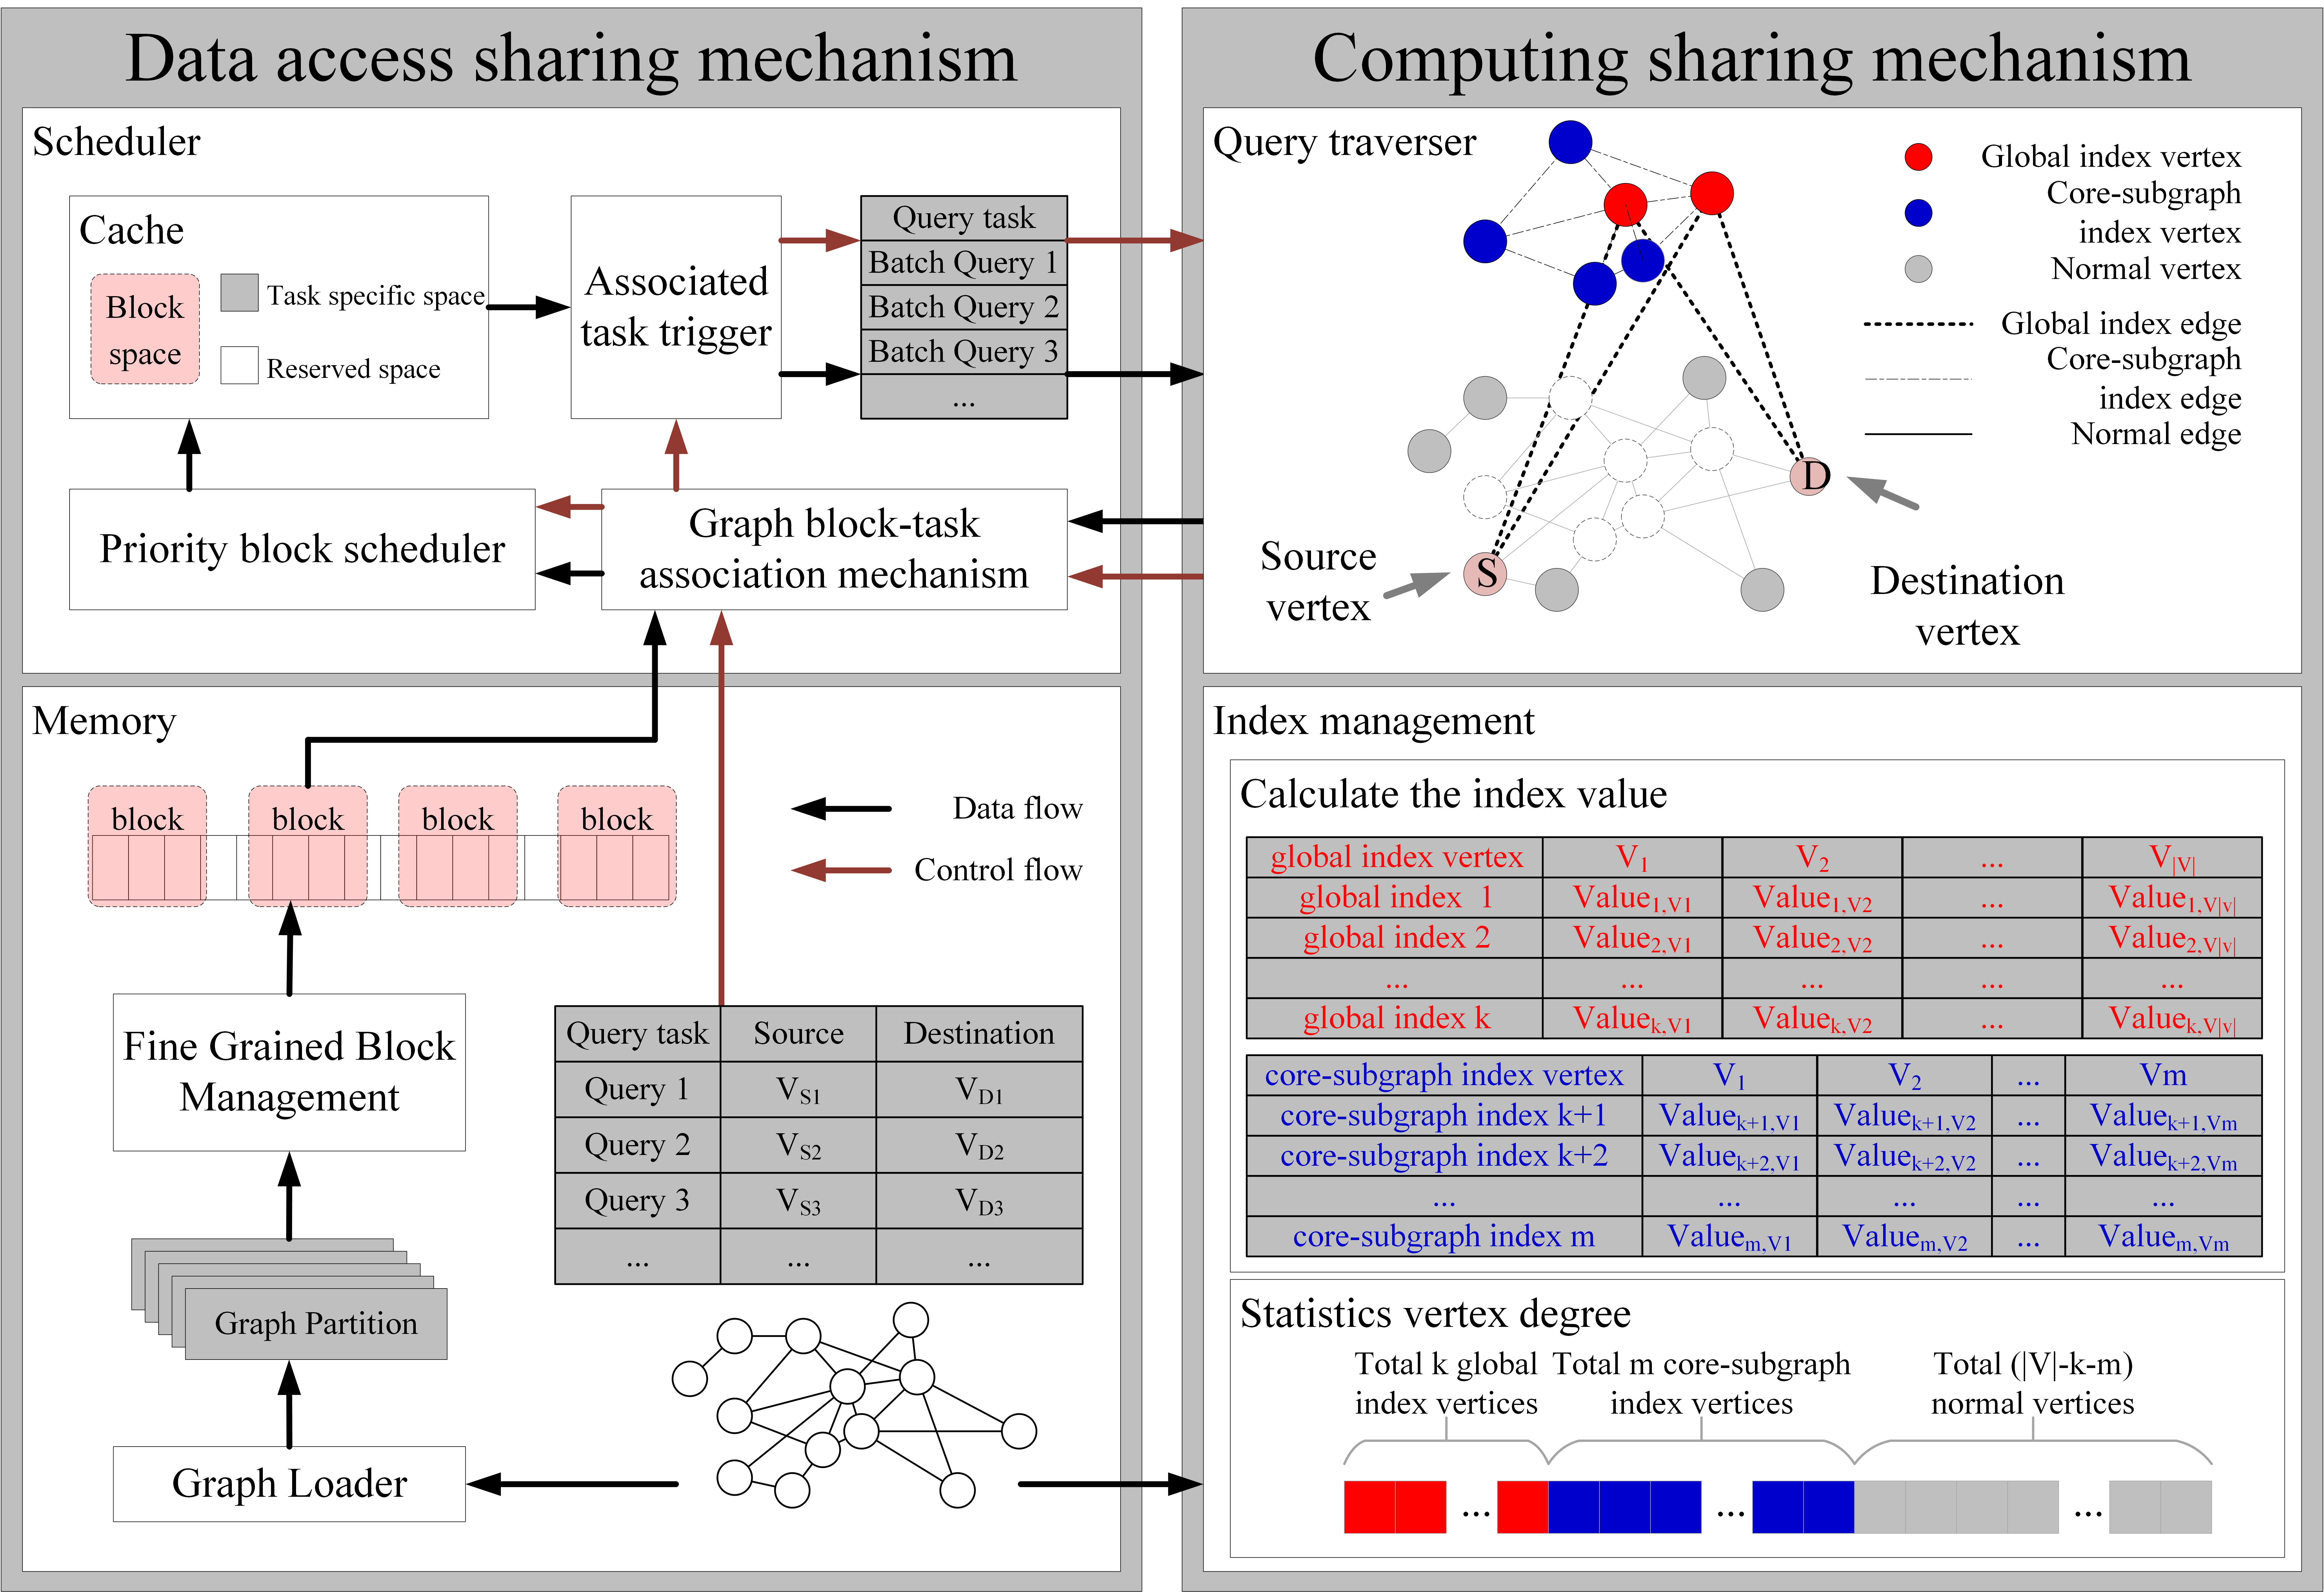
\includegraphics[width=\columnwidth]{系统架构.png}
    \caption{Your caption here}
    \label{fig:系统架构}
  \end{figure}
  

{\bf{Data Access Sharing Mechanism}}.Responsible for fine-grained sharing of graph structure data utilizing the data access similarity among concurrent tasks. Initially, it partitions the original graph data into coarse-grained graph partitions, distributed for parallel processing across different machines, similar to other distributed graph computing systems [xx]. Subsequently, a fine-grained chunk manager is employed to further divide coarse-grained graph partitions into fine-grained graph chunks. The association mechanism between graph chunks and tasks is then executed: if a query task qi has active vertices in a graph chunk bi, a relationship between qi and bi is established. The chunk priority scheduling mechanism prioritizes graph chunks with more associated tasks to be loaded into the Last Level Cache (LLC). The associated task trigger, based on active graph chunk information in LLC and chunk-task association information, selects all tasks with an association to execute in batch on shared graph chunks.

{\bf{Calculation Sharing Mechanism}}. It is responsible for leveraging dual-level index information (including global index and core subgraph index) to utilize computational similarity between concurrent query tasks for shared path computation. 1) Preprocessing Phase: It first gathers degree information for all vertices in the original graph data, sorts the vertices in descending order based on their degrees, and selects vertices ranked from 1 to k as global index vertices and vertices ranked from k+1 to k+m as core subgraph index vertices. 2) Index Building Phase: On one hand, before queries start, it executes a point-to-multipoint query algorithm to compute the best path values from global index vertices to all vertices in the graph (e.g., for PPSP tasks, it requires executing SSSP algorithm). For directed graphs, it calculates both the outbound and inbound path values for global index vertices, while for undirected graphs, only one calculation is needed. On the other hand, GraphCPP dynamically maintains the core subgraph through a runtime method. Specifically, any segment of a best path between a vertex pair corresponds to the best path between the corresponding vertices. Therefore, the core subgraph does not need precomputation for hot paths but dynamically explores hot paths after each query, adding them to the core subgraph structure. 3) Computation Sharing Phase: Global index vertices typically act as intermediaries for numerous paths, so at the beginning of a query, using global index vertices can compute the path value for a reachable path. This path may not necessarily be the best path between query vertex pairs but can provide a reference for pruning queries. Moreover, in pruning traversal based on upper bound + lower bound, global index can estimate the path value for query paths earlier, allowing earlier pruning of unsuitable paths. Using global index constitutes the first level of computation sharing. The core subgraph maintains best path values between hot vertices, serving as a highway network between query tasks. When a query task traverses hot vertices in the core subgraph, it connects to the highway. Leveraging the core subgraph, it can quickly reach the exit vertex from the entrance vertex without recalculating the path value for this hot path segment. Using the core subgraph constitutes the second level of computation sharing.


\subsection{Overall Execution Workflow}
Algorithm 1 outlines the comprehensive execution process of GraphCPP in handling concurrent query tasks. Assuming partitioning is completed, in the first line, we acquire the set \(block_table\), which includes all graph blocks on the current computing node, and the set \(Q\), which includes all query tasks on the current computing node. Each of them is allocated a segment of memory. In the second line, we enter a loop processing phase, and queries iterate until convergence is achieved. GraphCPP invokes \texttt{ChooseNextSharingBlock} to update the association between query tasks and graph blocks and selects the graph block \(b_i\) with the highest priority (having the most associated tasks). By tallying the associated blocks for each task (i.e., tasks with active vertices in the current block), we can determine all query tasks related to the current graph block \(b_i\) (fourth line). Next, we load \(b_i\) into the cache and parallelly process all associated query operations \(q_i\) (fifth line). This step embodies the idea of data sharing, i.e., multiple query tasks sharing the result of a single data access. Subsequently, we invoke \texttt{GraphCPPCompute} to perform point-to-point query operations \(q_i\) on the current block (details are provided in Section \ref{section:xx}). Iterative query task execution follows the Bulk Synchronous Parallel (BSP) model, where each iteration generates a new set of active vertices and updates to form a new query task (sixth line). If the new query remains associated with the current graph block \(b_i\), we add \(q_i\) to \(Q_{b_i}\) and return to the fifth line to continue querying on the graph block \(b_i\). Otherwise, it signifies that the new task is not associated with the current graph block, and it needs to be saved in the query task set; at this point, the task is suspended.

\begin{algorithm}
\caption{Concurrent Point-to-Point Queries}
\label{alg:concurrent_queries}
\begin{algorithmic}[1]

\Function{OverallWorkflow}{}
    \State \Call{MallocBuffers}{$block_table, Q$}
    \While{\Call{has\_active}{$block_table$}}
        \State $bi \gets$ \Call{ChooseNextSharingBlock}{}
        \State $Q_{bi} \gets$ \Call{ChooseAssociatedQueries}{$bi$}
        \For{\textbf{each} $qi \in Q_{bi}$} 
            \State $new\_query \gets$ \Call{GraphCPPCompute}{$qi, bi$}
            \If{\Call{has\_Associated}{$(bi, new\_query)$}}
                \State $Q_{bi}.\text{Push}(new\_query)$
            \Else
                \State $Q.\text{Push}(new\_query)$
            \EndIf
        \EndFor
    \EndWhile
\EndFunction

\end{algorithmic}
\end{algorithm}
  
The presented algorithm illustrates the overall workflow of GraphCPP. In the subsequent sections, we will delve into the detailed explanations of two optimization mechanisms: data access sharing and compute sharing.

\subsection{Data Access Sharing Mechanism}
In Section 2.2, we observed a significant overlap in graph structure data access among concurrent tasks. Under the existing processing mechanism, this overlapping data cannot be shared and utilized. However, for point-to-point query tasks on the graph, the order of data access does not affect the correctness of the results. The core idea of our data sharing mechanism is to transform the original "task → data" linear task scheduling order into a "data → task" fine-grained concurrent task scheduling order. This allows us to leverage data similarity among concurrent query tasks, distribute data access overhead, enhance cache utilization efficiency, and consequently, improve system throughput. We will address two key questions in the following sections: 1) How to determine the shared data segments? 2) How to implement data sharing among multiple tasks? Finally, we will describe additional measures to further exploit data access similarity.

\paragraph{Determine Shared Data Segments}

{\bf{Determine the granularity of shared graph partitions.}} Distributed memory graph computing systems need to load data into the cache to improve data access efficiency. Ideally, the data of shared graph partitions should fully fit into the Last-Level Cache (LLC) to avoid frequent eviction and reloading of different parts of partitions. However, the granularity of graph partitions should not be too small, as it would increase synchronization overhead in task processing. We use the formula x to determine an appropriate size for shared graph partitions. Here, $B_S$ represents the size of the graph structure data for the shared partition, $G_S$ represents the size of the graph structure data for the partition it belongs to, $|V|$ is the total number of vertices on the partitioned graph, $V_S$ represents the average space required to store state information for a vertex, $N$ is the number of concurrent query tasks, $LLC_S$ is the size of the LLC cache, and $R_S$ is the size of reserved redundant space. The two terms on the right side of the formula represent graph structure data and task-specific data, respectively (their sizes are proportional to the scale of the graph partition and the number of concurrent query tasks). The right side of the formula represents the size of the available space per task after deducting the reserved cache space. Using this formula, we determine the maximum granularity for each shared graph partition under the premise of adapting to LLC capacity.

\begin{equation}
    B_S + \frac{B_S}{G_S} \cdot \lvert V \rvert \cdot V_S \cdot N \leq LLC_S - R_S
    \end{equation}

{\bf{Logical Partitioning.}} Once the granularity of shared graph blocks is established, GraphCPP can proceed with the logical partitioning during the graph preprocessing phase. This process involves subdividing coarse-grained graph partitions on the distributed system into finer-grained shared graph blocks. Pseudocode for partitioning graph blocks in GraphCPP is presented in algorithm 2:

\begin{algorithm}
\caption{Logical Partition Algorithm}
\begin{algorithmic}[1]
\Function{Partition}{$P_i, block_table$}
    \State $block\_map \gets$ null
    \For{each $e \in P_i$}
        \If{$e.src$ in $block\_map$}
            \State $block\_map[e.src] \mathrel{+{+}}$
        \Else
            \State $block\_map[e.src] \gets 1$
        \EndIf
        \If{$\text{block\_map.size()} \geq B_S$}
            \State $block_table.\text{push}(block\_map)$
            \State $block\_map.\text{clear()}$
        \EndIf
    \EndFor
\EndFunction
\end{algorithmic}
\end{algorithm}

The logical partition function takes two parameters: one is the graph partition structure data $P_i$ recorded in edge table format, and the other is the set of graph blocks $block_table$ owned by the partition (Line 1). In Line 2, we utilize a dictionary structure called $block_map$ to collect information about graph blocks. Its key records the source vertex ID of an edge, and its value records the number of outgoing edges corresponding to that vertex. In Line 4, GraphCPP iterates through each edge in the partition. If the edge has already been loaded into the current partition, the count of outgoing edges for that partition is incremented (Line 6). If the vertex is added to the dictionary for the first time, the count of outgoing edges for the partition is set to 1 (Line 8). After processing each edge, there is a check to determine if the current block is full (Line 11). If the block is full, the current block is added to the $block_set $(Line 12), and the recorded block information is cleared (Line 13). This way, when all the data in the partition has been traversed, and each edge in the partition is assigned to a specific graph block, we obtain the collection of logically partitioned graph blocks.

\subsubsection{Share Similar Data Among Multiple Tasks}

Establishing the Association between Shared Blocks and Query Tasks. Through the previous steps, we have achieved fine-grained graph partitioning in a logical manner. Since this partitioning is only logical, the data remains contiguous on the physical storage medium. Therefore, it is easy to determine the partition in which a vertex is located based on its ID. During query execution, each task qi maintains an active vertex set $Set_{act,i}$ throughout the iterative computation process. It follows the updating strategy: 1) Initially, $Set_{act,i}$ only contains the source vertex Si of the query. 2) Process the active vertices in $Set_{act,i}$ according to the flow of the point-to-point query algorithm, removing the processed vertices from the active set. 3) If a vertex's state changes in this round and it is not pruned, add the vertex to $Set_{act,i}$ for processing in the next round. We first deduce the graph block to which a vertex belongs by reverse inference of its ID and then utilize a specially designed array to store the traversed partitions for each task. Since point-to-point queries adopt a pruning-based traversal strategy, the number of active vertices in each execution round is not high. Therefore, establishing the association between query tasks and their respective blocks can be done with relatively low overhead.

Determining the Priority of Partition Scheduling. After establishing the association between query tasks and their corresponding blocks, we can tally the number of tasks associated with each block. The higher the task count, the more tasks share the block, indicating greater benefits from processing this block. Consequently, blocks with a higher task count are prioritized for placement into the Last-Level Cache (LLC).

Triggering Concurrent Execution of Associated Tasks. Having obtained the shared graph data blocks, based on the association between shared blocks and query tasks, we can infer the active query tasks. These tasks share the graph structure data in the LLC, and we execute these query tasks using a batch computing approach. As shown in Algorithm X, active tasks generate new active vertices after one round of execution. If these new active vertices remain associated with the current shared block, the query tasks continue execution. Shared blocks always remain in the LLC until all query tasks associated with them are processed, at which point they are evicted.

\subsubsection{Batch Execute Similar Tasks}

At any given moment, there are numerous random query tasks in the concurrent task pool, each with significantly different optimal query paths. We observed that some tasks exhibit low similarity, meaning their query tasks have minimal overlap, and in some cases, no overlap at all. Conversely, there are tasks with high similarity, where, for instance, the path of query A includes the path of query B, and for query B, its path completely overlaps with query A. For our data sharing mechanism, the higher the overlap rate of paths, the more efficient the data access, resulting in fewer redundant synchronous iterations. To address this, we propose a batch execution strategy that is aware of similar tasks, selecting batches of similar tasks from the task pool for execution. This approach further leverages data and computation similarity. Specifically, GraphCPP randomly selects a query task from the task pool, retrieves the starting and destination vertices of the task, and performs BFS algorithm to obtain the neighbor vertex sets SetS for the starting vertex and SetD for the destination vertex. Note that, considering that some central nodes may have a large number of neighbor nodes, we set an upper limit of 500 for neighbor nodes. Subsequently, it traverses the task pool, filtering out all queries with starting points in SetS and destination points in SetD, treating them as similar tasks to be processed concurrently. It's important to note that if the starting or destination vertex of a query belongs to a high-degree vertex, indexing can be directly used to accelerate the query process without employing regular query steps. Excluding high-degree vertices, the overhead of the k-hop SSSP itself is minimal, and the execution process can be concurrent with regular queries, making the execution cost negligible.


\subsection{Computation Sharing Mechanism}

GraphCPP achieves two levels of computation sharing through the global index mechanism and the core subgraph index mechanism. The inherent overhead of a global index is significant, so in practice, a small number of hot vertices are often chosen to build a global index (typically around 16). However, due to the characteristics of a power-law distribution, these hot vertices act as intermediary hub nodes for different queries. As a result, for the majority of point-to-point queries, a path through the source vertex, global index vertex, and destination vertex can be found. Although ensuring that this path is always the optimal path for a query is challenging, it provides valuable reference values for pruning queries, realizing the first level of computation sharing. Furthermore, the core subgraph mechanism, without the need for preprocessing, explores the optimal paths based on existing query results, achieving computation sharing for hot paths. Compared to the global index, the core subgraph is more lightweight, allowing for a higher coverage range by increasing the number of hot vertices. This provides more accurate pruning bounds, accelerating the convergence speed of pruning queries. Algorithm 3 illustrates the pseudocode for the computation sharing mechanism.

\begin{algorithm}
    \caption{Shared Computation Algorithm}
    \begin{algorithmic}[1]
    
    \Function{IndexPreprocess}{$V, k, m$} 
        \State $global\_vertices, core\_subgraph\_vertices \gets \text{SortVerticesByDegree}(V, k, m)$
        \State $global\_index \gets \text{BuildGlobalIndex}(k)$
        \State $core\_subgraph\_index \gets \text{InitCoreSubgraph}(m, global\_index)$
    \EndFunction

    \Function{SharedComputation}{$global\_index, core\_subgraph\_index, query$}
        \State $bound \gets \text{FirstLevelSharing}(global\_index, query)$ 
        \While{$\text{activeVerticesCount} \neq 0$}
            \State $activeVertex \gets \text{GetNextActiveVertex}()$
            \If{$\text{activeVertex} \in \text{coreSubgraph}$}
                \State $\text{UpdateBounds}(bound, \text{SecondLevelSharing}\newline (core\_subgraph\_index, query))$
            \EndIf
            \For{each $neighbor$ of $\text{activeVertex}$}
                \State $\text{UpdateBoundsByNeighbors}(neighbor)$
            \EndFor
            \State $\text{activeVerticesCount} \gets \text{UpdateActiveVertices}()$
        \EndWhile
    \EndFunction

    \Function{MaintainCoreSubgraph}{$bestPath$}
        \State $hotPath \gets \text{ExtractHotPath}(bestPath)$
        \State $hotPathValue \gets \text{CalculateHotPathValue}(hotPath)$
        \State $\text{AddToCoreSubgraph}(hotPath, hotPathValue)$
    \EndFunction
    
    \end{algorithmic}
\end{algorithm}


The steps for implementing computation sharing are as follows:
1) Index Preprocessing (Lines 1-4):After sorting the degrees of vertices, the system selects the top $k+m$ hot vertices with the highest degrees. The first $k$ vertices serve as global index vertices (where $k$ is user-defined), and the remaining vertices become core subgraph vertices. The computation of the global index is completed during preprocessing. GraphCPP executes the SSSP algorithm to calculate the optimal paths (including index values and parent nodes) for $k$ high-degree vertices to all vertices in the graph. The results are stored in an array indexed by the high-degree vertices' IDs. The core subgraph omits the precomputation process, directly reusing the computation results of each query, requiring only initialization during preprocessing.
2) Computation Sharing (Lines 5-13): Global index vertices act as pivotal nodes for query paths. Most queries have at least one path passing through global index vertices. Although this path may not be the optimal path, it provides a reliable reference for query pruning. Therefore, before executing point-to-point queries, an approximate boundary is determined using the global index, representing the first level of computation sharing. Subsequently, an iterative query algorithm is executed, continuously processing new active vertices until all vertices converge. For each active vertex, it is determined whether it belongs to the core subgraph. Initially, the core subgraph is empty and does not participate in sharing. As query tasks execute, the core subgraph gradually accumulates more hot paths. When an active vertex belongs to the core subgraph, the hot path value for the corresponding starting vertex can be directly obtained through the core subgraph, avoiding redundant computation. Additionally, the core subgraph allows the query boundary to jump directly from one hot vertex to another through the hot path, accelerating the speed of point-to-point queries.
3) Maintain the Core Subgraph (Lines 14-17): To ensure the lightweight nature of the core subgraph, hot paths are not precomputed. Instead, a subset of hot paths is explored from existing optimal paths, reusing previous computation results. Clearly, any path between any two vertices on an optimal path is also an optimal path. Therefore, with minimal overhead, identifying hot vertices from existing results and calculating results between hot vertices using a prefix sum method is sufficient. To achieve this, traversal paths and path values from the source vertex to each intermediate point need to be retained during the query process. Since point-to-point queries inherently require calculating this information, the overhead is minimal. Through these steps, we achieve efficient data sharing using a lightweight core subgraph index.

\subsection{Update Mechanism}
In practical applications, the underlying graph traversed by query tasks often undergoes dynamic changes, involving edge additions ($e_{\text{add}}$) and edge deletions ($e_{\text{delete}}$). Changes in the graph structure data can lead to errors in index values. Therefore, when dynamic updates occur in the dynamic graph, we not only need to update the graph structure information but also dynamically update the indexes. Graph structure information update: GraphCPP stores the out-neighbor of each vertex using an adjacency list. Therefore, we only need to modify the adjacency list of the corresponding out-neighbors based on the source vertex information when an edge is added (or deleted). Index update: We adopt an incremental updating approach, sequentially updating the global index and core subgraph index, minimizing redundant computation costs during index updates.

The number of global index vertices is relatively small ($k$ global index vertices), but it records a substantial number of index values ($k \times |V|$ global index values). Therefore, index information can be stored on each vertex. Each vertex maintains two tables: $table1$ records the parent nodes on the optimal paths to $k$ global vertices, and $table2$ records the index values of the optimal paths from this vertex to $k$ global vertices. Incremental updates are performed on these two tables based on the type of edge update. Specifically, when an edge addition update ($e_{\text{add}}$) occurs, we first obtain the source vertex $src$, destination vertex $dst$, and the weight between the two points. We then sequentially check each global index vertex. If $Index_{\text{src}} + \text{weight} > Index_{\text{dst}}$, we update $parent_{\text{dst}}$ in $table1$ to $src$ and $Index_{\text{dst}}$ in $table2$ to $Index_{\text{src}} + \text{weight}$. Otherwise, there is no need to update the index for that global vertex. In the case of an edge deletion update, we check each global index vertex and determine if $parent_{\text{dst}}$ equals $src$. If true, it indicates that we have deleted the original optimal path to $dst$, and we need to recalculate $Index_{\text{dst}}$. Similar to other incremental computation methods, updates to $dst$ will gradually propagate outward, requiring updates for all downstream vertices on the optimal paths that pass through $dst$. If $parent_{\text{dst}}$ is not equal to $src$, there is no need to update that global index vertex.

The core subgraph index records a small number of indexes between high-degree vertices (up to $m \times m$ index values, where $m$ is significantly smaller than the graph data scale). Therefore, we use an independent two-dimensional array to store the core subgraph. Specifically, edge addition updates add to the existing graph structure, which may create new shortcuts, causing the original optimal paths to degenerate into non-optimal paths. For our pruning queries, non-optimal path indexes lead to early overestimation of boundary values. However, as the iteration progresses, point-to-point queries still traverse to more optimal paths, ultimately converging to the correct optimal paths. Extracting the latest hot path values from the converged paths completes the update to hot paths. For edge deletion updates, GraphCPP checks if both vertices of the deleted edge appear on some hot path. If yes, the original hot paths are interrupted, rendering all affected hot paths invalid. If only one vertex or no vertices appear on some hot path, the deleted edge does not affect hot paths, and there is no need for an update. Since the core subgraph index reuses the optimal path results from each query, no separate calculation is needed, resulting in overall low overhead.

The above mechanism implements incremental maintenance of graph structure data, global indexes, and core subgraph indexes. Considering that subtle graph updates do not significantly impact the overall computation results, we temporarily store subtle graph updates $\Delta G$ until its size exceeds a preset threshold or a certain time interval is reached. Only then do we execute batch graph update operations, further reducing update costs.

\section{EXPERIMENTAL EVALUATION}
\subsection{Experimental Setup}

{\bf{Hardware Configuration}}: The experiments were conducted on an 8-node cluster, with each machine equipped with 2 Intel Xeon E5-2680 v4 CPUs featuring 14 physical cores, 256 GB of memory, and a 35MB Last-Level Cache (LLC). All nodes were interconnected through an Infiniband network with a bandwidth of 300Gbps. The programs were compiled using gcc version 7.5.0, openMPI version 4.1.2, and with openMP enabled.
    
{\bf{Graph Algorithms}}: To maintain consistency with prior work [xx], we selected six different algorithms widely applied as benchmarks in various graph-related fields such as graph clustering, graph classification, and graph prediction. These algorithms fall into the categories of weighted graph algorithms and unweighted graph algorithms. 1) Weighted Graph Algorithms: Point-to-Point Shortest Path (PPSP), Point-to-Point Widest Path (PPWP), and Point-to-Point Narrowest Path (PPNP) are employed to find the shortest, widest, or narrowest path between two vertices. These algorithms have broad applications in areas such as social/financial networks, traffic planning, money laundering monitoring, and network quality analysis. 2) Unweighted Graph Algorithms: Breadth-First Search (BFS), Connectivity, and Reachability are three common pairwise queries on unweighted graphs. They are used to determine the shortest path between two vertices, check whether two vertices are connected in an undirected graph, and verify connectivity between two vertices in a directed graph, respectively. These algorithms are widely applied in advanced algorithms like bi-connectivity, higher-order connectivity, and graph clustering.

{\bf{Graph Datasets}}: The graph datasets used for the aforementioned algorithms are presented in Table x. LiveJournal and Twitter-2010 belong to social network graphs, while UK-2007-05 and Gsh-2015-host represent web-crawl graphs. These datasets exhibit power-law graphs with small diameters and skewed distributions, capturing real-world graph distribution scenarios. Our experiments are based on dynamic graphs, utilizing a snapshot mechanism where graph updates are performed on an unclosed snapshot, and graph queries are executed on a closed snapshot. Unclosed snapshots are periodically transformed into closed snapshots, replacing the original snapshot.

\begin{table}[h]
    \centering
    \begin{tabular}{lccc}
    \hline
    Datasets          & Vertices & Edges  & Data sizes \\
    \hline
    LiveJournal[1]    & 4.8M     & 69M    & 526MB      \\
    Twitter-2010[2]   & 41.7M    & 1.5B   & 10.9GB     \\
    Gsh-2015-host[3]  & 68.7M    & 1.8B   & 13.4GB     \\
    UK-2007-05[4]     & 106M     & 3.74B  & 27.9GB     \\
    \hline
    \end{tabular}
    \caption{Dataset Information}
    \end{table}

{\bf{System Comparison}}: We conducted a comparative analysis of GraphCPP's query performance with that of PnP, Tripoline, and SGraph. Since these systems are not open source, we re-implemented their mechanisms using the Gemini distributed graph processing framework. As none of these three systems inherently supports concurrent operations, we made modifications to enable them to handle multiple jobs simultaneously. We compared the performance of these systems in two modes: PnP-S, PnP-C, Tripoline-S, Tripoline-C, SGraph-S, and SGraph-C. In systems with the "-S" suffix, jobs are sequentially processed, while in those with the "-C" suffix, jobs are handled concurrently, managed by the operating system.

To evaluate performance, we submitted PPsP, PPWP, PPNP, BFS, Connectivity, and Reachability queries sequentially or concurrently until a specific number of jobs were generated. Parameters for each job were set randomly, even if they belonged to the same graph algorithm. For concurrent submissions, the intervals between job submissions were also randomized. Tripoline, SGraph, and GraphCPP employed a similar global index mechanism, with the global index set to 16 in our experiments. The core subgraph vertices in GraphCPP were set to 128. All benchmarks were executed 10 times, and the results are reported as average values.
    

\subsection{Overall Performance Comparison}
Figure 9 depicts the total execution time of xx concurrent jobs using different schemes. For conciseness, only the optimal results are displayed, and due to significant variations in the execution times of different test cases, we normalize the execution time relative to PnP's performance. It is evident that, for all graphs, GraphCPP achieves shorter execution times (and higher throughput) compared to the other schemes. In comparison to SGraph-S, SGraph-C, PnP-S, PnP-C, Tripoline-S, and Tripoline-C, GraphCPP demonstrates an average throughput improvement of approximately xx, xx, xx, xx, xx, and xx times, respectively. This enhancement in throughput is accomplished by reducing data access costs and efficiently pruning the core subgraph in GraphCPP.

To provide a more in-depth analysis of performance, we further divide the total time into data access time and graph processing time. As shown in Figure 10, GraphCPP requires less time for graph data access compared to other systems, and this proportion decreases further as the graph size increases. For example, in the case of Gsh-2015-host, GraphCPP's data access time is reduced by xx times to xx times compared to other systems. Two key factors contribute to GraphCPP's efficiency: 1) identical portions of graph data required by different concurrent jobs only need to load and maintain a single copy in memory, reducing memory consumption; 2) graph data blocks are prioritized and periodically loaded into the LLC based on the number of associated tasks, promoting job reuse and effectively lowering LLC miss rates, minimizing unnecessary memory data transfers. Additionally, thanks to the two-level computing sharing mechanism, GraphCPP's computation time is also lower than that of other systems.

\subsection{Efficiency of Data Access Sharing Mechanism}
GraphCPP employs a data sharing mechanism to reduce redundant data access. To qualitatively illustrate the efficiency of this mechanism, we evaluate the LLC utilization of different systems, and the results are presented in Figure 11. Notably, GraphCPP demonstrates lower LLC miss rates compared to the other six systems. In the case of UK-2007-05, GraphCPP's LLC miss rate is only xx, while SGraph-S, SGraph-C, PnP-S, PnP-C, Tripoline-S, and Tripoline-C exhibit LLC miss rates of xx, xx, xx, xx, xx, and xx, respectively. This is primarily attributed to GraphCPP allowing multiple jobs to share a single graph data copy in the LLC, enabling more efficient utilization of the LLC and enhancing data locality for jobs.

Additionally, we track the total amount of data swapped into the LLC by these 16 jobs. Generally, the concurrent execution mode (-C) tends to swap more data into the LLC compared to the sequential execution mode (-S). This is because concurrent jobs lack data sharing, leading to frequent swapping of graph data in and out of the LLC and resulting in more redundant memory data transfers. As illustrated in Figure 12, GraphCPP swaps significantly less data compared to SGraph-S, PnP-S, and Tripoline-S (xx, xx, and xx, respectively, in UK-2007-05). This reduction is attributed to GraphCPP maximizing the similarity in data access among concurrent tasks.

\subsection{Efficiency of the Computation Sharing Mechanism}
Figure x evaluates the temporal relationship between the graph processing time of each system. Due to significant differences in the graph processing time of each system, we represent the normalized time as the PnP graph processing time. PnP relies purely on pruning without utilizing an index, reducing preprocessing time but resulting in the longest query computation time. Tripoline, leveraging upper-bound pruning and a global index, reduces graph processing time. SGraph, employing upper-bound and lower-bound pruning strategies, achieves the best pruning effect, requiring the fewest calculated vertices and minimizing graph processing time. While the graph processing time of these three systems may fluctuate slightly based on different query characteristics, overall, the graph processing time remains stable. In contrast, GraphCPP's graph processing time initially aligns with SGraph, as it adopts a global index mechanism similar to SGraph. However, due to the continuous improvement of GraphCPP's core subgraph index mechanism during queries, it can leverage optimizations at the second level to continuously accelerate graph processing time, resulting in a reduction over time; GraphCPP shortens its processing time.

{\bf{Global Index Overhead}}: As the number of global indices increases, the time required for maintaining the indices also grows. In our experiments, PnP did not incur maintenance overhead for global indices as it did not utilize them. However, Tripoline, SGraph, and GraphCPP employed similar global index mechanisms. As shown in Figure x, GraphCPP's index construction overhead is comparable to other systems due to the adoption of the same number of global indices. Nevertheless, GraphCPP achieves higher throughput, allowing it to handle more queries in the same time frame, thereby distributing the global index overhead.

{\bf{Core Subgraph Index Overhead}}: We evaluated the impact of the core subgraph index on GraphCPP's performance. With the global index set to 16, GraphCPP-128, GraphCPP-256, and GraphCPP-without represent versions with core subgraph indices of 128, 256 vertices, and without using core subgraph indices, respectively. Table x illustrates the memory space occupied by these three versions of core subgraphs. It is noticeable that GraphCPP-128 and GraphCPP-256 incur only a minimal increase in memory usage compared to GraphCPP-without, all maintaining 16 global indices. This minimal increase is attributed to the fact that core subgraph vertices only store distances to other core subgraph vertices, requiring very little additional space compared to global indices storing distances to all vertices.

Moreover, Table x displays the total execution time of GraphCPP-128, GraphCPP-256, and GraphCPP-without across 16 jobs. Consistently, GraphCPP-256 and GraphCPP-128 outperform GraphCPP-without, with GraphCPP-256 being faster than GraphCPP-128. On Friendster, the processing times of GraphCPP-256 and GraphCPP-128 are only xx and xx times that of GraphCPP-without, respectively. This improvement is attributed to the additional core subgraph vertices enhancing pruning effectiveness and constraining upper and lower bounds.

{\bf{Update Maintenance Overhead}}: Tripoline, SGraph, and GraphCPP share a common global index mechanism, with an equal global index number set to 16. GraphCPP, additionally implementing a second level of sharing through the core subgraph mechanism, incurs additional maintenance overhead. As described in Section xxx, during edge addition updates, there is no need to specifically update the corresponding core subgraph hot paths. In the case of edge deletion updates, only the affected hot paths need to be deleted. Since we do not perform a dedicated computation for the core subgraph but rather extract hot paths from existing results, graph updates only affect the accuracy of the core subgraph mechanism without incurring expensive update maintenance overhead.


\subsection{Scalability of GraphCPP}
Figure 16 illustrates the performance comparison between GraphCPP and six other systems under varying numbers of concurrent PPsP jobs. GraphCPP exhibits superior performance improvement as the number of concurrent jobs increases. For 2, 4, 8, and 16 concurrent jobs, GraphCPP achieves acceleration ratios of xx, xx, xx, and xx, respectively, in comparison to SGraph-S. This improvement stems from GraphCPP's amortization, which saves more data access and storage costs with an increasing number of jobs. It's important to note that with only one concurrent job, GraphCPP's fine-grained scheduling operations do not occur, resulting in minimal differences in execution time compared to other schemes. According to our tests, the block scheduling cost of GraphCPP constitutes only xx-xx\% of the total execution time. Furthermore, due to resource contention, the performance of the concurrent version (-C) is considerably worse than both GraphCPP and the sequential version (-S). Therefore, a simple modification of existing graph processing systems to support concurrent tasks might not be an optimal choice.

Next, we assess the horizontal scalability of GraphCPP. To achieve this goal, we initially increase the number of CPU cores on a single node to evaluate GraphCPP's execution time with 16 PPsP jobs. As depicted in Figure 17, GraphCPP consistently outperforms other schemes, especially when the number of cores is higher. This is attributed to the shared graph data among concurrent tasks in GraphCPP, reducing data access costs compared to other schemes. Additionally, we evaluate the performance of different schemes on 1, 2, 4, and 8 nodes. As shown in Figure 18, GraphCPP's performance on 8 nodes is xx-xx times that of a single machine, indicating robust scalability. Moreover, GraphCPP's scalability surpasses that of SGraph, PnP, and Tripoline due to lower communication costs facilitated by data sharing and core subgraph indexing. Consequently, we believe that GraphCPP can efficiently support practical point-to-point query applications.

\section{RELATED WORK}
{\bf{Graph Processing Systems}}: With the increasing prominence of graph computing as a research focus, a plethora of graph computing systems of diverse types have emerged. 1)Single-node in-memory graph computing systems: Ligra [x] accelerates graph computation, especially graph traversal algorithms, by switching between push and pull computation modes. KickStarter [x] and GraphBolt [x] implement incremental processing for streaming graphs. DiGraph [x] proposes an efficient iterative directed graph processing system on GPUs. LCCG [x], DepGraph [x], and TDGraph [x] utilize topology-aware execution methods, reducing redundant computation and data access costs; 2) Single-node out-of-core graph computing systems: GraphChi [x] and X-Stream [x] achieve efficient out-of-core graph processing through sequential storage access. FlashGraph [x] employs a semi-external memory graph engine, achieving high IOPS and parallelism. GridGraph [x] improves locality and reduces I/O operations. DGraph [x] accelerates graph processing through faster state propagation. GraphM [x] adopts a data-sharing approach, optimizing throughput for concurrent systems; 3) Distributed graph computing systems: Pregel [x] introduces the Bulk Synchronous Parallel (BSP) computation model, addressing the processing needs of graphs with billions of edges in terms of performance, scalability, and fault tolerance. PowerGraph [x] proposes a "vertex-cut" graph partitioning approach, effectively reducing communication volume and addressing load imbalance caused by high-degree vertices. PowerLyra [x] employs a hybrid computing model, using different computation strategies for high-degree and low-degree vertices. Gemini [x] introduces a dual-mode computation engine, ensuring scalability while maintaining performance. CGraph [x] uses a data-centric Load-Trigger-Pushing (LTP) model, leveraging temporal and spatial similarities between concurrent tasks to reduce distributed system overhead; While the aforementioned works are designed for general graph algorithms, point-to-point query algorithms, focusing on specific vertex pairs' graph relationships, exhibit significant differences. Point-to-point query algorithms, through pruning strategies, can greatly enhance execution efficiency. However, general graph computing systems do not inherently support such algorithms.

{\bf{Point-to-Point Queries}}: Previous studies have delved into extensive research on point-to-point queries. Notably, $Hub^2$ [x] introduced a specialized accelerator with a hub-centric approach, emphasizing the challenges posed by vertices with a high degree of connections, or hubs, in expanding the search space for shortest path calculations. To address this, it proposed the hub-Network concept, limiting the search scope of hub nodes and accelerating the PPSP process through online pruning. However, due to the specialized nature of $Hub^2$'s dedicated accelerator, its applicability is constrained. PnP observed the traversal process of point-to-point queries and introduced an upper-bound-based pruning strategy, reducing unnecessary vertex traversals and providing a fresh perspective for point-to-point query research. Tripoline integrated both indexing and pruning, employing the triangle inequality principle to achieve incremental evaluation of point-to-point queries without prior knowledge. SGraph optimized pruning strategies further, using upper and lower bounds based on the triangle inequality principle, achieving sub-second query response times on large graphs. Despite these advancements, these systems predominantly concentrate on enhancing the speed of individual point-to-point queries, overlooking the substantial load posed by large-scale concurrent queries.

{\bf{Concurrent Graph Computing}}: Various graph computing systems have explored the realm of concurrent computing. GraphM identified "data access similarity" among concurrent graph computing tasks and proposed a data-centric scheduling strategy to facilitate data sharing between multiple tasks, enhancing the throughput of concurrent graph computing. However, GraphM is a single-machine out-of-core graph computing system using the BSP computing model, limited to static graphs. Building upon this, CGraph[x] extended the application scenarios to distributed dynamic graph computing systems, optimizing communication mechanisms and load balancing strategies for distributed scenarios. Despite these advancements, it remains an out-of-core system, not well-suited for high-load concurrent query scenarios, even with the distribution of disk access costs across different subgraphs through scheduling strategies. ForkGraph efficiently conducts concurrent graph processing in memory, employing a concession-based scheduling strategy, handling only a portion of the data in each iteration to accelerate overall execution speed. Nevertheless, it is a single-machine in-memory system, not specifically optimized for point-to-point queries, making it unsuitable for executing concurrent point-to-point query tasks on massive datasets.


\section{CONCLUSION}
The existing point-to-point query systems primarily focus on optimizing the speed of individual queries, neglecting the optimization of throughput for concurrent queries. This paper identifies strong data access similarity and computation similarity among concurrent point-to-point query tasks. It proposes a data-driven concurrent point-to-point query system, GraphCPP. By employing a data-driven caching execution mechanism, GraphCPP achieves overlapping data access sharing among concurrent queries. Simultaneously, through a two-level computation sharing mechanism, it better realizes computation sharing among multiple tasks. Experimental results indicate that GraphCPP's performance surpasses that of the state-of-the-art graph query systems, including SGraph[x], Tripoline[x], and Pnp[x], by a factor of XXX.

\section{ACKNOWLEDGMENTS}


\begin{thebibliography}{1} %这里的1是指用最多的数字有几位,比如10就是指用最多的数字有两位

\bibitem{ams} %这行是指把这个参考文献标签为ams,这个标签可以自己取,作用是在正文中引用时用的
{\it{Mathematics into Type}}, American Mathematical Society. Online available:  %\it的意思是把后面的内容变成斜体

\bibitem{oxford} %这行是指把这个参考文献标签为oxford
T.W. Chaundy, P.R. Barrett and C. Batey, {\it{The Printing of Mathematics}}, Oxford University Press. London, 1954.

\bibitem{lacomp}{\it{The \LaTeX Companion}}, by F. Mittelbach and M. Goossens

\bibitem{mmt}{\it{More Math into LaTeX}}, by G. Gr\"atzer

\bibitem{amstyle}{\it{AMS-StyleGuide-online.pdf,}} published by the American Mathematical Society

\bibitem{Sira3}
H. Sira-Ramirez. ``On the sliding mode control of nonlinear systems,'' \textit{Systems \& Control Letters}, vol. 19, pp. 303--312, 1992.

\bibitem{Levant}
A. Levant. ``Exact differentiation of signals with unbounded higher derivatives,''  in \textit{Proceedings of the 45th IEEE Conference on Decision and Control}, San Diego, California, USA, pp. 5585--5590, 2006.

\bibitem{Cedric}
M. Fliess, C. Join, and H. Sira-Ramirez. ``Non-linear estimation is easy,'' \textit{International Journal of Modelling, Identification and Control}, vol. 4, no. 1, pp. 12--27, 2008.

\bibitem{Ortega}
R. Ortega, A. Astolfi, G. Bastin, and H. Rodriguez. ``Stabilization of food-chain systems using a port-controlled Hamiltonian description,'' in \textit{Proceedings of the American Control Conference}, Chicago, Illinois, USA, pp. 2245--2249, 2000. %这里的\textit是指把后面的内容变成斜体

\end{thebibliography} %这个是参考文献的结束

\begin{IEEEbiographynophoto}{Jane Doe} %这里的Jane Doe是指作者的名字
Biography text here without a photo.
\end{IEEEbiographynophoto} %这个是作者的结束

\begin{IEEEbiography}[{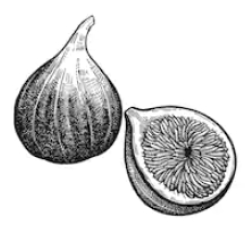
\includegraphics[width=1in,height=1.25in,clip,keepaspectratio]{fig1.png}}]{IEEE Publications Technology Team}
In this paragraph you can place your educational, professional background and research and other interests.\end{IEEEbiography} %这行的作用是插入作者的照片


\end{document}


